\documentclass[serif, aspectratio=169]{beamer}
%\documentclass[serif]{beamer}  % for 4:3 ratio

\usepackage[T1]{fontenc} 
\usepackage[utf8]{inputenc}
\usepackage{fourier} % see "http://faq.ktug.org/wiki/uploads/MathFonts.pdf" for other options
\usepackage{hyperref}
\usepackage{latexsym,amsmath,xcolor,multicol,booktabs,calligra}
\usepackage{graphicx,pstricks,listings,stackengine}
\usepackage{lipsum}
\usepackage{../HKUSTstyle}

%imports customs%
\usepackage{caption}    % for subfigures
\usepackage{subcaption} % for subfigures
\usepackage{ragged2e}
\usepackage{booktabs,makecell}
\usepackage{colortbl}
\usepackage{multirow}
\usepackage{cite}
\usepackage{tcolorbox}
\usepackage[sort,authoryear]{natbib}

\author{Julien Bezançon}

\title{Découverte du Traitement Automatique des Langues}
\subtitle{CM 2~: Tâches classiques du TAL et leurs applications}

\institute{julien.bezancon@univ-lorraine.fr / \url{https://julienbez.github.io}}

\date{}

% defs
\def\cmd#1{\texttt{\color{red}\footnotesize $\backslash$#1}}
\def\env#1{\texttt{\color{blue}\footnotesize #1}}

% set colors
\definecolor{hkustyellow}{RGB}{167, 131, 55}
\definecolor{hkustblue}{RGB}{0, 56, 116}
\definecolor{hkustred}{RGB}{209, 51, 59}

% easy colors
\newcommand{\tred}[1]{\textcolor{red!50}{#1}}
\newcommand{\tgreen}[1]{\textcolor{green}{#1}}
\newcommand{\tyellow}[1]{\textcolor{yellow}{#1}}
\newcommand{\tpurple}[1]{\textcolor{purple!50}{#1}}

% CLI environment
\newenvironment{CLI} % Command Line Interface
    {
    \noindent
    \ttfamily 
    \footnotesize
    \begin{tcolorbox}[colback=gray!150,colframe=black]
    \color{white}
    \begin{tabular}{p{4.5cm}p{7.5cm}}
    }
    { 
    \end{tabular}
    \end{tcolorbox}
    }

% Exercice environment
\newenvironment{exoframe}
    {
    \setbeamercolor{background canvas}{bg=hkustblue}
    \renewcommand\thefootnote{\textcolor{white}{\arabic{footnote}}}
    \color{white}
    \setbeamercolor{structure}{fg=white}
    \begin{frame}
    }
    {
    \end{frame}
    }

\lstset{
    basicstyle=\ttfamily\small,
    keywordstyle=\bfseries\color{deepblue},
    emphstyle=\ttfamily\color{deepred},    % Custom highlighting style
    stringstyle=\color{deepgreen},
    numbers=left,
    numberstyle=\small\color{halfgray},
    rulesepcolor=\color{red!20!green!20!blue!20},
    frame=shadowbox,
}

\begin{document} %  --- --- --- --- --- --- --- --- --- --- --- --- 

\begin{frame}[noframenumbering,plain]
    \titlepage
    \vspace*{-0.6cm}
    \begin{figure}[htpb]
        \begin{center}
            \hspace{0.3cm}
            
\includegraphics[width=0.7\columnwidth]{../../../IMAGES/loria_idmc.png}
        \end{center}
    \end{figure}
\end{frame}

% \begin{frame}    
%     \tableofcontents[sectionstyle=show,
%     subsectionstyle=show/shaded/hide,
%     subsubsectionstyle=show/shaded/hide]
% \end{frame}

\section{Introduction}

\begin{frame}{Les applications du TAL}
    \begin{block}{Avec le TAL, on peut mettre en place~:}
        \begin{itemize}
            \item des agents conversationnels
            \item des systèmes de filtrage de spams
            \item des assistants vocaux
            \item des outils de correction automatique
            \item des outils de résumé automatique
            \item etc
        \end{itemize}
    \end{block}
    \begin{center}
        \Large
        Pour réussir à mettre en place ces applications, \\ il faut d'abord les découper en tâches
    \end{center}
\end{frame}

\begin{frame}{Un exemple}
    \begin{figure} %TODO : trouver ref
        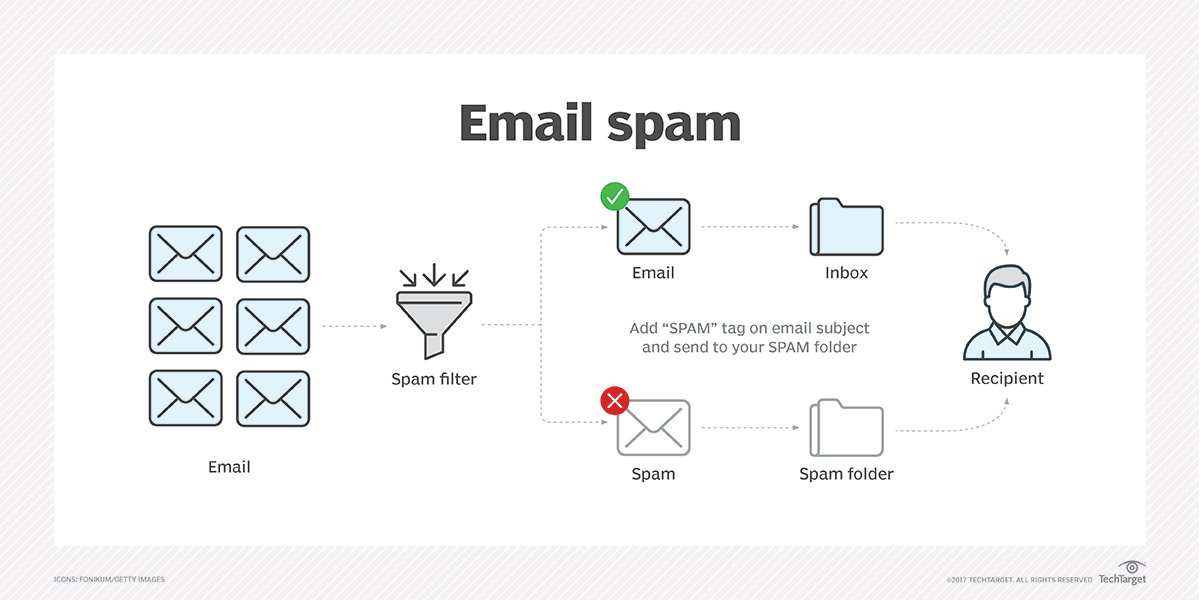
\includegraphics[width=0.8\columnwidth]{../../../FIGURES/découverte_tal/mail_spam_filter.jpg}
        \caption*{Source~: un article d'Andrew Zola\footnote{\url{https://www.techtarget.com/cybersecurity/definition/spam-filter}}}
    \end{figure}
\end{frame}

\begin{frame}{Un exemple}
    \begin{block}{Un mail est un spam si...}
        \begin{itemize}
            \item il contient le mot "urgent" \hfill $\Rightarrow$ recherche d'information
            \item un riche héritier a besoin d'argent \hfill $\Rightarrow$ analyse sémantique
            \item le domaine mail de l'envoyeur est inconnu \hfill $\Rightarrow$ base de données
            \item il est envoyé 50 fois en 2 heures \hfill $\Rightarrow$ similarité
            \item etc \hfill ...
        \end{itemize}
    \end{block}
\end{frame}

\begin{frame}{Les tâches du TAL}
    \begin{block}{Le TAL se découpe en une multitude de tâches}
        \begin{itemize}
            \item Classification de données
            \item Extraction d'information
            \item Traduction automatique
            \item Analyse syntaxique
            \item Systèmes de Q\&A
            \item Big Data
            \item etc
        \end{itemize}
    \end{block}
    \begin{center}
        \Large
        Pourquoi existe-t-il autant de tâches en TAL ?
    \end{center}
\end{frame}

\begin{frame}{Les tâches du TAL}
    \begin{block}{Rappel~: le langage est naturel}
        \begin{itemize}
            \item Redondant, ambigu, implicite
            \item Phénomènes linguistiques (néologie, coréférence, etc)
            \item Machine $\neq$ Humain
        \end{itemize}
    \end{block}
    \begin{center}
        \Large
         La séparation en tâches n'est qu'une façon \\ d'avancer sans devoir se préoccuper de tout à la fois.
    \end{center}
    \begin{center}
        \Large
         Il existe BEAUCOUP de phénomènes linguistiques.
    \end{center}
\end{frame}

\begin{frame}{Pour résumer...}
    \begin{block}{Tâche}
        \begin{itemize}
            \item Définie par les scientifiques
            \item Cherche à répondre à une problématique précise
            \item Restreinte au cadre de la recherche (?)
        \end{itemize}
    \end{block}
    \begin{block}{Application}
        \begin{itemize}
            \item Définie par des individus
            \item Cherche à répondre à un "besoin"
            \item Combine généralement plusieurs tâches
        \end{itemize}
    \end{block}
    \begin{center}
        \Large
        Dans ce cours, nous nous intéressons aux tâches du TAL.
    \end{center}
\end{frame}

% Tache : classification de textes
% Application : ranger des récits par catégorie, détecter des spams, trier des textes par langue, ...

% Tache : recherche d'information
% Application : moteur de recherche, fouille dans des jeux de données, système de recommandation

% Tache : reconnaissance d'entités nommées
% Application : recherche de noms de médicaments dans des textes cliniques, veille informatique, résumé automatique

% Tache : Analyse automatique d'image
% Application : système de détection de tumeur, tri d'images 

% Tache : Synthèse de la parole
% Application : assistants vocaux, dictée vocale, recherche vocale

% Tache : désidentification
% Application : anonymisation ou pseudonymisation de données sensibles

% Tache : NER et entity linking (pas de bon équivalent fr ?)
% Application : mise en relation de données, création d'ontologies, moteurs de recherche

% Tache : correction syntaxique
% Application : corrige tout ce que vous écrivez sur un ordi

% Tache : traduction automatique
% Application : multiples et self-explanatory

% Tache : Analyse en parties du discours
% Application : contribue à améliorer de nombreuses tâches portant sur le texte

\end{document}
